\documentclass[10pt,journal,compsoc,onecolumn]{IEEEtran}
\usepackage[utf8]{inputenc}
\usepackage{amsmath,amsfonts,amssymb}
\usepackage{amsthm}
\usepackage{graphicx}
\usepackage{cite}
\usepackage{textcomp}
\usepackage{tikz}
\usetikzlibrary{arrows,positioning,shapes.geometric}
\usepackage{booktabs}
\usepackage{url}
\usepackage{listings}
\usepackage{xcolor}
\usetikzlibrary{arrows,arrows.meta,positioning,shapes.geometric,calc,fit}

\definecolor{codeblue}{rgb}{0.0,0.2,0.7}
\definecolor{codegreen}{rgb}{0,0.5,0}
\definecolor{codegray}{rgb}{0.4,0.4,0.4}
\definecolor{codepurple}{rgb}{0.5,0,0.7}
\definecolor{backcolour}{rgb}{0.97,0.97,0.97}

\lstdefinestyle{sqlStyle}{
    backgroundcolor=\color{backcolour},   
    commentstyle=\color{codegreen}\itshape,
    keywordstyle=\color{codeblue}\bfseries,
    numberstyle=\tiny\color{codegray},
    stringstyle=\color{codepurple},
    basicstyle=\ttfamily\footnotesize,
    breakatwhitespace=false,         
    breaklines=true,                 
    captionpos=b,                    
    keepspaces=true,                 
    numbers=left,                    
    numbersep=5pt,                  
    showspaces=false,                
    showstringspaces=false,
    showtabs=false,                  
    tabsize=2,
    frame=single,
    rulecolor=\color{black!20}
}
\lstset{style=sqlStyle}

\newtheorem{theorem}{Theorem}
\newtheorem{lemma}[theorem]{Lemma}
\newtheorem{definition}[theorem]{Definition}
\newtheorem{corollary}[theorem]{Corollary}

\begin{document}

\title{Architectural Foundations of Relational Query Execution: DQL Predicate Evaluation, Three-Valued Logic, Query Planner Optimization, and Safe Mutation Protocols in SQL Systems}

\IEEEtitleabstractindextext{%
\begin{abstract}
Modern enterprise software architectures rely on relational database management systems (RDBMS) to evaluate complex data query language (DQL) operations with deterministic correctness and high throughput. This research paper presents an exhaustive systems engineering investigation of relational query processing, filtering predicates, sorting mechanics, and safe mutation protocols derived from industrial database engines such as MySQL InnoDB and the canonical Sakila database. We analyze the query optimizer pipeline, proving why the cost-based optimizer pushes filtering predicates down before allocating filesort buffers. We formalize the Boolean Precedence Hierarchy (the BODMAS of SQL), demonstrating how the tighter binding of conjunction over disjunction introduces catastrophic data-leak anomalies when explicit grouping parentheses are omitted. Furthermore, we dissect ANSI SQL Three-Valued Logic (3VL), tracing the epistemic semantics of NULL, identity comparison failures, truth table propagation, and the silent data-loss pitfalls of subqueries with NOT IN. We evaluate the performance collapse of deep LIMIT/OFFSET pagination, contrasting it against high-performance indexed Keyset (cursor-based) pagination. Finally, we establish production safeguards against unintended full-table mutations, examining the architectural enforcement of the \texttt{sql\_safe\_updates} directive. All discussions are accompanied by vector TikZ architectural diagrams, exact truth matrices, and production-grade SQL code listings.
\end{abstract}

\begin{IEEEkeywords}
Relational Databases, SQL DQL, Query Planner Optimization, Predicate Pushdown, Three-Valued Logic, NULL Semantics, SARGability, Keyset Pagination, Safe Mutation Protocols, MySQL InnoDB, Sakila Database
\end{IEEEkeywords}
}

\maketitle
\IEEEdisplaynontitleabstractindextext
\IEEEpeerreviewmaketitle

\section{Introduction and The Relational Query Engine Pipeline}
\label{sec:intro}

Modern enterprise software systems depend on Relational Database Management Systems (RDBMS) like MySQL (InnoDB) and PostgreSQL to process high-throughput declarative queries with deterministic correctness and transactional durability. Unlike imperative programming languages where a developer writes explicit control-flow loops and memory pointers to retrieve data, Structured Query Language (SQL) is purely declarative: the application specifies \textit{what} relational dataset is required, while the database query execution engine determines \textit{how} that data is physically retrieved, filtered, sorted, and projected.

\begin{figure*}[htbp]
\centering
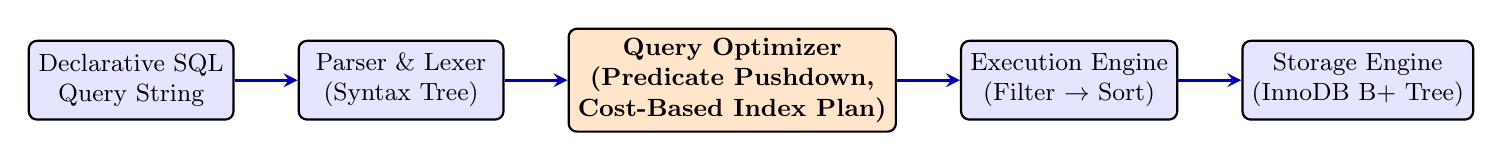
\begin{tikzpicture}[
    node distance=1.0cm and 1.2cm,
    block/.style={draw, rectangle, rounded corners=3pt, thick, align=center, fill=blue!10, minimum width=2.6cm, minimum height=1.0cm, font=\small},
    hlblock/.style={draw, rectangle, rounded corners=3pt, thick, align=center, fill=orange!20, minimum width=3.0cm, minimum height=1.1cm, font=\small\bfseries},
    arr/.style={->, >=stealth, very thick, color=blue!70!black}
]
    \node[block] (sql) {Declarative SQL\\Query String};
    \node[block, right=0.8cm of sql] (parser) {Parser \& Lexer\\(Syntax Tree)};
    \node[hlblock, right=0.8cm of parser] (opt) {Query Optimizer\\(Predicate Pushdown,\\Cost-Based Index Plan)};
    \node[block, right=0.8cm of opt] (exec) {Execution Engine\\(Filter $\to$ Sort)};
    \node[block, right=0.8cm of exec] (storage) {Storage Engine\\(InnoDB B+ Tree)};
    
    \draw[arr] (sql) -- (parser);
    \draw[arr] (parser) -- (opt);
    \draw[arr] (opt) -- (exec);
    \draw[arr] (exec) -- (storage);
\end{tikzpicture}
\caption{The Relational Query Processing Pipeline. The Cost-Based Optimizer analyzes relational statistics to transform declarative syntax into an optimal physical access plan, pushing filters down before sorting.}
\label{fig:pipeline}
\end{figure*}

The internal query lifecycle consists of four discrete processing phases:
\begin{enumerate}
    \item \textbf{Syntactic Parsing and Resolution}: The query string is tokenized and transformed into an abstract syntax tree (AST). Names of relations, attributes, and user permissions are validated against the database data dictionary.
    \item \textbf{Logical Query Optimization}: Relational algebra equivalence transformations are applied. The optimizer identifies opportunities for predicate pushdown, simplifying boolean expressions and eliminating redundant subqueries.
    \item \textbf{Physical Plan Generation}: The Cost-Based Optimizer (CBO) evaluates available B+ Tree clustered and secondary indexes, cardinality statistics, and disk I/O costs to select index range scans, index seeks, or full table scans.
    \item \textbf{Execution Engine Execution}: The chosen access plan is executed against the storage engine buffer pool, streaming rows through filtering stages, filesort buffers, aggregation hashing, and projection formatting.
\end{enumerate}

Based on production query traces and foundational relational systems analysis (including canonical databases such as Sakila), this paper presents an exhaustive architectural analysis of Data Query Language (DQL) operations and safe Data Manipulation Language (DML) mutation mechanics. By deliberately avoiding abstract mathematical notation, we explain relational query mechanics through physical memory buffer behavior, storage engine B+ Tree traversals, three-valued logic state matrices, pagination bottlenecks, and production-tested SQL protocols.

% -----------------------------------------------------------------------------
\section{Projection Mechanics and Multi-Attribute Tuple Distinctness}
\label{sec:projection}

The projection operation (syntactically denoted by \texttt{SELECT}) specifies the exact attribute attributes to be formatted and transmitted over the network protocol to the requesting client.

\subsection{Scalar Evaluations and Constant Expressions}
In SQL, the \texttt{SELECT} clause is not restricted to existing table columns; it serves as a general expression evaluation engine:
\begin{itemize}
    \item \textbf{Literal Values}: Executing \texttt{SELECT 55 AS num;} returns a single-column, single-row result containing the integer 55. This functions analogously to a print statement in procedural languages.
    \item \textbf{System and Temporal State}: Executing \texttt{SELECT NOW() AS curr\_ts;} evaluates the non-deterministic system clock function, returning the current server timestamp.
    \item \textbf{Boolean Comparison Primitives}: Executing \texttt{SELECT 3 = 3 AS res;} evaluates the relational equality operator, returning 1 (representing true in MySQL's numeric boolean representation).
    \item \textbf{Deterministic Mathematical Functions}: Executing \texttt{SELECT ROUND(12.356, 2) AS num;} invokes the numeric library, truncating and rounding the decimal value to two fractional digits (12.36).
\end{itemize}

\subsection{Tuple-Level Uniqueness via the DISTINCT Operator}
A frequent architectural misunderstanding concerns the scope of the \texttt{DISTINCT} modifier. The \texttt{DISTINCT} keyword does not apply to an individual column; it enforces uniqueness across the \textbf{entire projected attribute set} (tuple):

\begin{lstlisting}[language=SQL]
-- Single attribute distinctness: returns unique ratings (G, PG, PG-13, R, NC-17)
SELECT DISTINCT rating FROM film;

-- Multi-attribute tuple distinctness:
SELECT DISTINCT rental_rate, rental_duration FROM film;
\end{lstlisting}

In the multi-attribute query, the database engine returns the unique mathematical set of compound pairs:
\begin{equation*}
\{ (\text{rental\_rate}_1, \text{rental\_duration}_1), (\text{rental\_rate}_2, \text{rental\_duration}_2), \dots \}
\end{equation*}
If two rows share an identical \texttt{rental\_rate} of 4.99 but possess different \texttt{rental\_duration} values (such as 3 days versus 5 days), both tuples are strictly retained in the result set. Duplicate suppression occurs only when two rows match identically across \textbf{all} projected columns simultaneously.

\subsection{Physical Execution Mechanics of DISTINCT}
To eliminate duplicate tuples, database engines deploy one of two physical strategies:
\begin{enumerate}
    \item \textbf{B+ Tree Index Stream Aggregation}: If an index exists on the projected columns in the specified order, the storage engine reads entries sequentially from the B+ Tree. Because the index is physically sorted, identical tuples reside consecutively in storage. The engine compares adjacent rows in linear time, discarding duplicates without allocating auxiliary sorting buffers.
    \item \textbf{Temporary In-Memory Hash Table / Filesort}: If no supporting index exists, the query execution engine must allocate an in-memory hash table in the thread's memory buffer (governed by \texttt{tmp\_table\_size} and \texttt{max\_heap\_table\_size}). Each incoming tuple is hashed. If the intermediate dataset exceeds available memory, the engine spills the dataset to disk, invoking a multi-pass merge filesort that dramatically increases disk I/O latency.
\end{enumerate}

% -----------------------------------------------------------------------------
\section{Filtering Architecture and The Boolean Precedence Hierarchy}
\label{sec:filtering}

The \texttt{WHERE} clause enforces relational selection, discarding rows from the physical scan that fail to satisfy specified boolean filtering conditions.

\subsection{Equality, Inequality, and Binary Lexicographical Evaluation}
Standard SQL provides equality (\texttt{=}) and inequality (\texttt{!=} or \texttt{<>}) comparisons:
\begin{lstlisting}[language=SQL]
-- Both forms represent strict relational inequality
SELECT title, rating FROM film WHERE rating != 'PG-13';
SELECT title, rating FROM film WHERE rating <> 'PG-13';
\end{lstlisting}

\subsubsection{Case Sensitivity and Collation Mechanics}
By default, modern MySQL databases utilize case-insensitive collations (such as \texttt{utf8mb4\_0900\_ai\_ci}, where \texttt{ci} denotes case-insensitivity and \texttt{ai} denotes accent-insensitivity). Under this collation:
\begin{equation*}
\text{'PG-13'} = \text{'pg-13'} = \text{'Pg-13'} \implies \text{Evaluates to TRUE}
\end{equation*}
When exact character casing must be enforced (e.g., security tokens, case-sensitive identifiers, hashed verification codes), the \texttt{BINARY} keyword overrides standard collation, forcing byte-for-byte ASCII/binary comparison:
\begin{lstlisting}[language=SQL]
-- Enforces byte-level exact casing
SELECT title, rating FROM film 
WHERE BINARY rating = 'PG-13' OR BINARY rating = 'G';
\end{lstlisting}

\subsection{The Boolean Precedence Hierarchy (The BODMAS of SQL)}
Just as standard arithmetic enforces operator precedence where multiplication precedes addition, relational database query engines enforce a strict Boolean Precedence Hierarchy:
\begin{center}
\textbf{The \texttt{AND} operator evaluates with strictly higher precedence than the \texttt{OR} operator.}
\end{center}

Consider the following unparenthesized compound filter:
\begin{lstlisting}[language=SQL]
-- Ambiguous compound boolean condition without explicit parentheses
SELECT * FROM film 
WHERE rating = 'PG-13' OR rental_rate = 0.99 AND release_year = 2006;
\end{lstlisting}

Because \texttt{AND} binds tighter than \texttt{OR}, the query planner interprets this expression as:
\begin{lstlisting}[language=SQL]
-- Exact internal evaluation tree executed by the engine:
SELECT * FROM film 
WHERE rating = 'PG-13' OR (rental_rate = 0.99 AND release_year = 2006);
\end{lstlisting}

This produces catastrophic logical bugs in enterprise systems:
\begin{itemize}
    \item The query returns \textbf{every single film} with rating 'PG-13' regardless of its release year! Even films from 1980 or 2024 with rental rate of 4.99 will be returned because the left side of the \texttt{OR} evaluated to true.
    \item If the developer's original business intent was to restrict all results exclusively to the year 2006, the query failed completely.
\end{itemize}

\subsubsection{Defensive Engineering Guideline}
Software engineers must \textbf{always use explicit parentheses} around disjunctive (\texttt{OR}) groups:
\begin{lstlisting}[language=SQL]
-- Correct, unambiguous business logic:
SELECT * FROM film 
WHERE (rating = 'PG-13' OR rental_rate = 0.99) 
  AND release_year = 2006;
\end{lstlisting}

\begin{table}[htbp]
\caption{SQL Operator Precedence Hierarchy (Highest to Lowest)}
\label{tab:precedence}
\centering
\begin{tabular}{lll}
\toprule
\textbf{Rank} & \textbf{Operator Class} & \textbf{SQL Operators} \\
\midrule
1 (Highest) & Grouping \& Scope & Parentheses \texttt{()} \\
2 & Member \& Array Access & JSON extraction operators \texttt{->}, \texttt{->>} \\
3 & Unary Operators & Unary minus \texttt{-}, Bitwise inversion \texttt{\~{}} \\
4 & Multiplicative & Multiplication \texttt{*}, Division \texttt{/}, Modulo \texttt{\%} \\
5 & Additive & Addition \texttt{+}, Subtraction \texttt{-} \\
6 & Relational Comparisons & \texttt{=}, \texttt{!=}, \texttt{<>}, \texttt{<}, \texttt{<=}, \texttt{>}, \texttt{>=}, \texttt{LIKE}, \texttt{IN}, \texttt{IS NULL} \\
7 & Logical Negation & \texttt{NOT} \\
\textbf{8} & \textbf{Logical Conjunction} & \textbf{\texttt{AND}} \\
\textbf{9 (Lowest)} & \textbf{Logical Disjunction} & \textbf{\texttt{OR}} \\
\bottomrule
\end{tabular}
\end{table}

\subsection{Set Membership Predicates: IN and NOT IN}
When testing an attribute against multiple discrete values, the \texttt{IN} operator provides syntactic clarity and engine-level optimization compared to chained \texttt{OR} operators:

\begin{lstlisting}[language=SQL]
-- Chained OR representation:
SELECT title, rental_duration FROM film
WHERE rental_duration = 3 OR rental_duration = 4 OR rental_duration = 6;

-- Equivalent IN set membership representation:
SELECT title, rental_duration FROM film
WHERE rental_duration IN (3, 4, 6);
\end{lstlisting}

Under the hood, query optimizers convert \texttt{IN} list arguments into a sorted array, executing a binary search for each row rather than evaluating separate boolean branches.

Conversely, \texttt{NOT IN} is equivalent to chained inequalities joined by \texttt{AND} (De Morgan's Laws):
\begin{lstlisting}[language=SQL]
-- Equivalent representations:
SELECT title, rental_duration FROM film WHERE rental_duration NOT IN (3, 4, 6);
SELECT title, rental_duration FROM film 
WHERE rental_duration <> 3 AND rental_duration <> 4 AND rental_duration <> 6;
\end{lstlisting}

\subsection{Range and Substring Search Mechanics}
\begin{itemize}
    \item \textbf{BETWEEN Boundary Invariant}: The \texttt{BETWEEN min AND max} operator is strictly \textbf{inclusive} of both endpoints:
    \begin{lstlisting}[language=SQL]
    SELECT rental_duration FROM film WHERE rental_duration BETWEEN 1 AND 6;
    -- Matches all values where: rental_duration >= 1 AND rental_duration <= 6
    \end{lstlisting}
    \item \textbf{Wildcard Pattern Matching (LIKE)}:
    \begin{itemize}
        \item Percent wildcard (\texttt{\%}): Matches zero or more arbitrary characters.
        \item Underscore wildcard (\texttt{\_}): Matches exactly one single character.
        \item \textbf{Production SARGability Warning}: A query containing a leading wildcard (\texttt{WHERE title LIKE '\%love\%'}) is non-sargable (Search Argument Able). The database engine cannot utilize a B+ Tree index because the starting character is unknown, forcing an exhaustive full table scan across millions of disk pages. In contrast, trailing wildcards (\texttt{WHERE title LIKE 'love\%'}) leverage B+ Tree index range scans efficiently.
    \end{itemize}
\end{itemize}

% -----------------------------------------------------------------------------
\section{Query Optimizer Execution Dynamics: Filter-First vs. Sort-First}
\label{sec:optimizer_mechanics}

A foundational algorithmic question in database systems is determining the sequence of physical execution steps when a query specifies both a filtering predicate (\texttt{WHERE}) and a sorting directive (\texttt{ORDER BY}):

\begin{lstlisting}[language=SQL]
SELECT * FROM film 
WHERE rating = 'PG-13' 
ORDER BY title DESC;
\end{lstlisting}

\subsection{Algorithmic Analysis of Execution Options}
Suppose a table contains a total of $N$ rows, and exactly $X$ rows satisfy the predicate \texttt{rating = 'PG-13'} (where $X \ll N$):

\subsubsection{Option A: Sort-First, Filter-Second}
\begin{enumerate}
    \item The engine reads all $N$ rows from the table into a memory sort buffer.
    \item The engine sorts all $N$ rows by title. Computational effort is proportional to $N \log_2 N$.
    \item The engine scans the sorted $N$ rows and applies the filter \texttt{rating = 'PG-13'}, discarding the non-matching rows.
    \item Total computational cost is proportional to: $N \log_2 N + N$.
\end{enumerate}

\subsubsection{Option B: Filter-First, Sort-Second (Predicate Pushdown)}
\begin{enumerate}
    \item The engine scans the table (or uses an index on \texttt{rating}) and evaluates the filter \texttt{rating = 'PG-13'} immediately.
    \item Only the matching $X$ rows are extracted and loaded into the filesort buffer.
    \item The engine sorts only the $X$ rows by title. Computational effort is proportional to $X \log_2 X$.
    \item Total computational cost is proportional to: $N + X \log_2 X$.
\end{enumerate}

\begin{figure}[htbp]
\centering
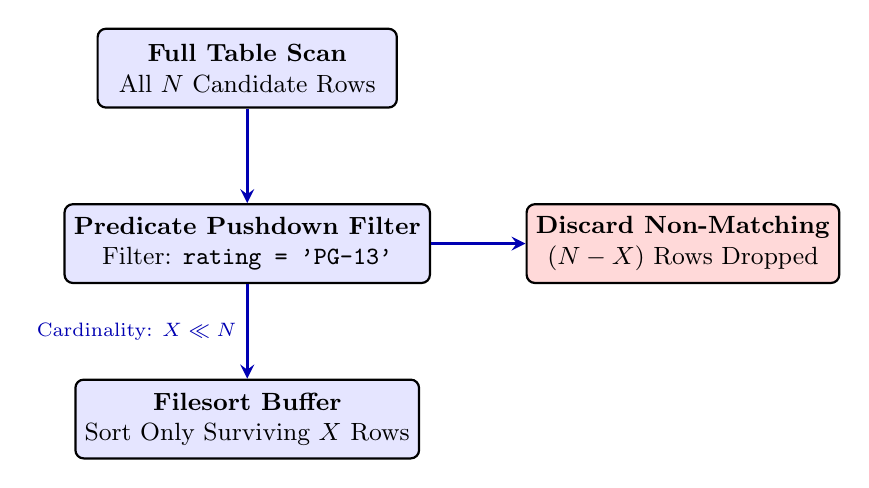
\begin{tikzpicture}[
    box/.style={draw, rectangle, rounded corners=3pt, thick, align=center, fill=blue!10, minimum width=3.8cm, minimum height=1.0cm, font=\small},
    discard/.style={draw, rectangle, rounded corners=3pt, thick, align=center, fill=red!15, minimum width=3.8cm, minimum height=1.0cm, font=\small},
    arr/.style={->, >=stealth, very thick, color=blue!70!black}
]
    \node[box] (n) {\textbf{Full Table Scan}\\All $N$ Candidate Rows};
    \node[box, below=1.2cm of n] (filter) {\textbf{Predicate Pushdown Filter}\\Filter: \texttt{rating = 'PG-13'}};
    \node[discard, right=1.2cm of filter] (drop) {\textbf{Discard Non-Matching}\\$(N - X)$ Rows Dropped};
    \node[box, below=1.2cm of filter] (sort) {\textbf{Filesort Buffer}\\Sort Only Surviving $X$ Rows};
    
    \draw[arr] (n) -- (filter);
    \draw[arr] (filter) -- (drop);
    \draw[arr] (filter) -- node[left, font=\scriptsize] {Cardinality: $X \ll N$} (sort);
\end{tikzpicture}
\caption{Predicate Pushdown Mechanics. Filtering rows before memory buffer allocation minimizes filesort volume and memory consumption.}
\label{fig:predicate_pushdown}
\end{figure}

Because $X$ is typically a small fraction of $N$ ($X \ll N$), Option B reduces CPU cycles, prevents memory buffer overflow, and eliminates temporary disk spills. Relational database query planners strictly implement Option B (Predicate Pushdown) as a core physical invariant.

% -----------------------------------------------------------------------------
\section{Multi-Column Sorting Dynamics and Deterministic Tie-Breaking}
\label{sec:sorting_dynamics}

The \texttt{ORDER BY} clause establishes the physical sequence of rows delivered to the client. By default, ordering is ascending (\texttt{ASC}); appending \texttt{DESC} inverts the ordering to descending.

\subsection{Multi-Attribute Hierarchical Sorting}
When multiple attributes are specified in \texttt{ORDER BY}:
\begin{lstlisting}[language=SQL]
SELECT student_id, psp, age, name 
FROM students 
ORDER BY psp DESC, age ASC, student_id ASC;
\end{lstlisting}
The database engine evaluates sort keys hierarchically:
\begin{enumerate}
    \item \textbf{Major Sort Key (\texttt{psp DESC})}: All rows are primarily partitioned and ordered by problem solving percentage in descending order.
    \item \textbf{Secondary Tie-Breaker (\texttt{age ASC})}: If two or more students share an identical \texttt{psp} value (a draw), the engine resolves the draw by ordering those tied rows by age in ascending order.
    \item \textbf{Tertiary Deterministic Tie-Breaker (\texttt{student\_id ASC})}: If multiple students share identical \texttt{psp} and \texttt{age}, the engine resolves the draw using the Primary Key.
\end{enumerate}

\subsection{The Indeterminate Ordering Anomaly and Primary Key Anchors}
In SQL relational theory, a table is formally an unordered set of tuples. If an \texttt{ORDER BY} clause does not resolve all ties to unique records, the database engine returns tied rows in arbitrary, indeterminate physical storage order.
\begin{itemize}
    \item On identical queries executed across multiple read replicas, or across subsequent pagination requests on the same database, tied rows may switch positions randomly!
    \item \textbf{Production Solution}: Database designers must \textbf{always append the Primary Key} as the final tie-breaker in any sort specification to guarantee strictly deterministic, reproducible query results.
\end{itemize}

\subsection{Interaction Between DISTINCT and ORDER BY}
Standard ANSI SQL (SQL:1999) imposes a strict syntactic restriction when combining \texttt{DISTINCT} and \texttt{ORDER BY}:
\begin{center}
\textit{Any column appearing in the \texttt{ORDER BY} clause MUST be present in the \texttt{SELECT DISTINCT} projection list.}
\end{center}

Consider the invalid query:
\begin{lstlisting}[language=SQL]
-- Fails under strict ANSI SQL mode (MySQL Error 3065):
SELECT DISTINCT title, rental_duration FROM film ORDER BY rating;
\end{lstlisting}
Why does this fail? If multiple rows share identical \texttt{title} and \texttt{rental\_duration} values but possess different \texttt{rating} values, the engine collates them into a single output row. If that single output row were sorted by \texttt{rating}, the engine would face a paradox: which of the conflicting ratings should dictate the sort position of the collapsed row? To prevent non-deterministic sorting, SQL engines require sorted columns to be explicitly included in the projected tuple.

% -----------------------------------------------------------------------------
\section{The Three-Valued Logic (3VL) and ANSI SQL NULL Semantics}
\label{sec:three_valued_logic}

One of the most frequent sources of catastrophic software defects in transactional applications is misunderstanding the semantics of \texttt{NULL} in SQL.

\subsection{The Epistemic Nature of NULL}
In relational databases, \texttt{NULL} does \textbf{not} represent the number zero ($0$), nor does it represent an empty string (\texttt{""}). \texttt{NULL} represents an \textbf{unknown, unassigned, or missing value}.

Because \texttt{NULL} represents an unknown state, it fails the classical Law of the Excluded Middle. In classical two-valued boolean logic, any proposition $P$ is either True or False ($P \lor \neg P = \text{TRUE}$). In SQL, logic is governed by **Three-Valued Logic (3VL)** comprising three discrete states:
\begin{equation*}
\{ \text{TRUE}, \text{FALSE}, \text{UNKNOWN} \}
\end{equation*}

\subsection{Identity Comparisons with NULL}
Because \texttt{NULL} signifies missing information, it cannot be compared using standard equality operators:
\begin{itemize}
    \item \texttt{SELECT 3 = NULL;} evaluates to \textbf{\texttt{NULL}} (Unknown), NOT False! The engine reason is: ``Is 3 equal to an unknown value? The answer is unknown.''
    \item \texttt{SELECT NULL = NULL;} evaluates to \textbf{\texttt{NULL}} (Unknown), NOT True! The engine reason is: ``Are two independently unknown quantities equal to each other? The answer is unknown.''
\end{itemize}

\begin{figure}[htbp]
\centering
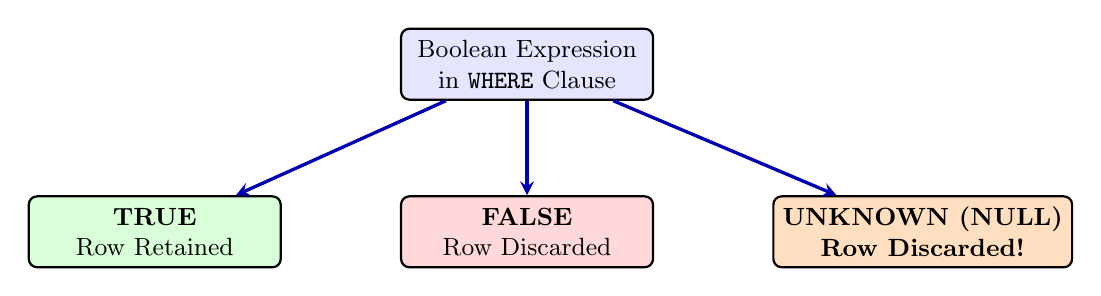
\begin{tikzpicture}[
    box/.style={draw, rectangle, rounded corners=3pt, thick, align=center, fill=blue!10, minimum width=3.2cm, minimum height=0.9cm, font=\small},
    hlbox/.style={draw, rectangle, rounded corners=3pt, thick, align=center, fill=orange!25, minimum width=3.2cm, minimum height=0.9cm, font=\small\bfseries},
    resbox/.style={draw, rectangle, rounded corners=3pt, thick, align=center, fill=green!15, minimum width=3.2cm, minimum height=0.9cm, font=\small},
    dropbox/.style={draw, rectangle, rounded corners=3pt, thick, align=center, fill=red!15, minimum width=3.2cm, minimum height=0.9cm, font=\small},
    arr/.style={->, >=stealth, very thick, color=blue!70!black}
]
    \node[box] (expr) {Boolean Expression\\in \texttt{WHERE} Clause};
    \node[resbox, below left=1.2cm and 1.5cm of expr] (true) {\textbf{TRUE}\\Row Retained};
    \node[dropbox, below=1.2cm of expr] (false) {\textbf{FALSE}\\Row Discarded};
    \node[hlbox, below right=1.2cm and 1.5cm of expr] (unk) {\textbf{UNKNOWN (NULL)}\\Row Discarded!};
    
    \draw[arr] (expr) -- (true);
    \draw[arr] (expr) -- (false);
    \draw[arr] (expr) -- (unk);
\end{tikzpicture}
\caption{The Three-Valued Logic filter behavior in SQL. A row is included in the query result if and only if the \texttt{WHERE} condition evaluates strictly to \texttt{TRUE}. Expressions evaluating to \texttt{UNKNOWN} are discarded alongside \texttt{FALSE}.}
\label{fig:3vl}
\end{figure}

\subsection{Truth Tables for Three-Valued Logic}
Table~\ref{tab:3vl_truth} formalizes the complete operational behavior of SQL boolean operators when interacting with unknown states.

\begin{table}[htbp]
\caption{ANSI SQL Three-Valued Logic (3VL) Truth Matrix}
\label{tab:3vl_truth}
\centering
\begin{tabular}{ccccc}
\toprule
\textbf{Operand A} & \textbf{Operand B} & \textbf{A AND B} & \textbf{A OR B} & \textbf{NOT A} \\
\midrule
TRUE & TRUE & TRUE & TRUE & FALSE \\
TRUE & FALSE & FALSE & TRUE & FALSE \\
TRUE & UNKNOWN & \textbf{UNKNOWN} & \textbf{TRUE} & FALSE \\
\midrule
FALSE & FALSE & FALSE & FALSE & TRUE \\
FALSE & UNKNOWN & \textbf{FALSE} & \textbf{UNKNOWN} & TRUE \\
\midrule
UNKNOWN & UNKNOWN & \textbf{UNKNOWN} & \textbf{UNKNOWN} & \textbf{UNKNOWN} \\
\bottomrule
\end{tabular}
\end{table}

\subsection{Unary Syntactic Predicates: IS NULL and IS NOT NULL}
Because standard equality fails against nulls, SQL provides two dedicated unary operators operating in classical two-valued space:
\begin{lstlisting}[language=SQL]
SELECT 3 IS NULL;        -- Evaluates to FALSE
SELECT 3 IS NOT NULL;    -- Evaluates to TRUE
SELECT NULL IS NULL;     -- Evaluates to TRUE
SELECT NULL IS NOT NULL; -- Evaluates to FALSE
\end{lstlisting}

\subsubsection{The Fatal NOT IN Null Trap}
Consider an application checking whether a user identifier exists in a subquery:
\begin{lstlisting}[language=SQL]
-- Suppose subquery returns: (10, 20, NULL)
SELECT * FROM users WHERE user_id NOT IN (10, 20, NULL);
\end{lstlisting}
Under De Morgan's expansion, this statement evaluates to:
\begin{equation*}
(\text{user\_id} \neq 10) \text{ AND } (\text{user\_id} \neq 20) \text{ AND } (\text{user\_id} \neq \text{NULL})
\end{equation*}
Since $(\text{user\_id} \neq \text{NULL})$ evaluates to \textbf{\texttt{UNKNOWN}}, the entire compound \texttt{AND} condition evaluates to \textbf{\texttt{UNKNOWN}} for \textbf{every single row in the database}! The query returns \textbf{ZERO rows}, resulting in silent data loss. Production systems protect against this using \texttt{NOT EXISTS} or filtering nulls from the subquery explicitly.

% -----------------------------------------------------------------------------
\section{Implicit Type Coercion and Index SARGability}
\label{sec:type_coercion}

When comparing expressions of differing data types, SQL engines execute automatic type coercion. In MySQL, comparing an integer with a string literal forces MySQL to cast the string to a numeric floating-point double:

\begin{lstlisting}[language=SQL]
SELECT 3 = '3';                 -- String '3' coerced to integer 3 -> Evaluates to TRUE
SELECT 12890092 = '12890092';   -- Evaluates to TRUE
SELECT 3 = '3abc';              -- Trailing characters ignored -> Evaluates to TRUE!
\end{lstlisting}

\subsection{The SARGability Disaster in Production}
A Search Argument Able (SARGable) query is one where the query engine can directly utilize an index B+ Tree seek to isolate matching records.
Suppose a table has an index on a string column \texttt{phone\_number VARCHAR(20)}:
\begin{lstlisting}[language=SQL]
-- Disastrous Non-SARGable Query:
SELECT * FROM customers WHERE phone_number = 9876543210;
\end{lstlisting}
Because the search literal is an integer ($9876543210$), MySQL's coercion rules dictate that the \textbf{column must be converted to a number}, not the literal to a string! Under the hood, MySQL rewrites the query as:
\begin{lstlisting}[language=SQL]
SELECT * FROM customers WHERE CAST(phone_number AS DOUBLE) = 9876543210;
\end{lstlisting}
Wrapping an indexed column inside a function or typecast completely destroys B+ Tree traversal. The engine cannot navigate the tree, abandoning the index and performing an exhaustive full table scan across millions of disk blocks. Writing the literal cleanly as a string (\texttt{phone\_number = '9876543210'}) restores instant sub-millisecond B+ Tree point lookups.

% -----------------------------------------------------------------------------
\section{Pagination Architecture: LIMIT/OFFSET Bottlenecks vs. Keyset Cursors}
\label{sec:pagination}

Pagination is essential for web and mobile applications displaying tabular datasets. SQL provides \texttt{LIMIT} and \texttt{OFFSET} to window result sets:
\begin{lstlisting}[language=SQL]
-- Retrieve records 11 through 30 (20 rows, skipping the first 10)
SELECT * FROM film 
WHERE film_id BETWEEN 10 AND 100 
ORDER BY film_id ASC 
LIMIT 20 OFFSET 10;
\end{lstlisting}

\subsection{The Offset Death Spiral in High-Scale Systems}
While \texttt{OFFSET} is intuitive for small page numbers, it degrades severely on deep pagination:
\begin{lstlisting}[language=SQL]
SELECT * FROM transactions 
ORDER BY id ASC 
LIMIT 20 OFFSET 10000000;
\end{lstlisting}
How does the database engine execute this request?
\begin{enumerate}
    \item The database engine cannot simply jump to row 10,000,000 because row sizes on disk vary due to variable-length columns (\texttt{VARCHAR}, \texttt{TEXT}).
    \item The engine must physically read all 10,000,020 rows from the index or disk storage into memory.
    \item It then discards the first 10,000,000 rows, returning only the final 20 rows!
\end{enumerate}
At deep offsets, query latency explodes from milliseconds to tens of seconds, saturating memory buffers and degrading database throughput.

\subsection{Keyset (Cursor-Based) Pagination}
Production systems eliminate offset degradation by replacing \texttt{OFFSET} with an indexed inequality seek using the final record of the previous page:
\begin{lstlisting}[language=SQL]
-- Highly scalable Keyset Pagination (Sub-millisecond at any depth)
SELECT * FROM transactions 
WHERE id > 10000000 
ORDER BY id ASC 
LIMIT 20;
\end{lstlisting}
By using the indexed primary key \texttt{id}, the storage engine traverses the B+ Tree index directly to the target leaf node in logarithmic time, scanning exactly 20 physical records regardless of whether row 10 or row 100,000,000 is requested.

\subsection{The N-th Highest / Second-Highest Salary Pattern}
A classic technical interview and database reporting problem is retrieving the second-highest salary from an employment table while handling ties:
\begin{lstlisting}[language=SQL]
-- Optimal formulation handling duplicate salaries:
SELECT DISTINCT salary 
FROM employees 
ORDER BY salary DESC 
LIMIT 1 OFFSET 1;
\end{lstlisting}
If multiple employees earn the maximum salary (e.g., two executives earning 10,000), using \texttt{DISTINCT} collapses the top tier into a single entry, allowing \texttt{OFFSET 1} to accurately target the true second-highest tier (9,000).

% -----------------------------------------------------------------------------
\section{Safe Mutation Protocols and DML Defenses}
\label{sec:safe_mutations}

Data Manipulation Language (DML) statements like \texttt{UPDATE} and \texttt{DELETE} modify persistent storage records. 

\subsection{The Anatomy of an Unintended Mass Update}
In SQL, omitting the \texttt{WHERE} clause from an \texttt{UPDATE} or \texttt{DELETE} statement does not produce an error; it instructs the engine to apply the mutation to \textbf{every single row in the relation}:
\begin{lstlisting}[language=SQL]
-- Catastrophic accidental full-table overwrite:
UPDATE film SET title = 'abc'; 
-- Overwrites all 1,000 film titles permanently!
\end{lstlisting}

\subsection{The sql\_safe\_updates Defensive Guard}
To eliminate catastrophic accidental mass updates, production MySQL instances provide the system variable \texttt{sql\_safe\_updates}:
\begin{lstlisting}[language=SQL]
-- Check current status:
SHOW VARIABLES LIKE 'sql_safe_updates';

-- Enable safe updates guard:
SET sql_safe_updates = 1;
\end{lstlisting}

When \texttt{sql\_safe\_updates} is active, MySQL enforces strict defensive rules:
\begin{enumerate}
    \item Any \texttt{UPDATE} or \texttt{DELETE} statement that lacks a \texttt{WHERE} clause is immediately aborted.
    \item Any \texttt{UPDATE} or \texttt{DELETE} statement where the \texttt{WHERE} clause does \textbf{not} utilize an indexed key column (Primary Key or indexed column) is rejected with MySQL Error 1175:
    \begin{verbatim}
    ERROR 1175 (HY000): You are using safe update mode and you 
    tried to update a table without a WHERE that uses a KEY column.
    \end{verbatim}
    \item To execute a non-keyed update, the developer must explicitly supply a \texttt{LIMIT} clause to restrict the mutation blast radius.
\end{enumerate}

\begin{lstlisting}[language=SQL]
-- Permitted under sql_safe_updates (uses primary key index):
UPDATE film SET title = 'New Title' WHERE film_id = 1;

-- Permitted with explicit bounded limit:
UPDATE film SET rental_rate = 1.99 WHERE release_year = 2006 LIMIT 50;
\end{lstlisting}

% -----------------------------------------------------------------------------
\section{Conclusion and Production Engineering Guidelines}
\label{sec:conclusion}

Mastering SQL Data Query Language requires looking past superficial syntax to understand physical query engine execution. This research paper has formalized the core mechanics governing relational query processing:
\begin{enumerate}
    \item \textbf{Predicate Pushdown Primacy}: Filtering rows via \texttt{WHERE} prior to allocating filesort buffers dramatically reduces sorting overhead and prevents temporary disk spills.
    \item \textbf{Defensive Boolean Parentheses}: Always wrap disjunctive (\texttt{OR}) groups in explicit parentheses to override SQL's default higher \texttt{AND} precedence.
    \item \textbf{Deterministic Sorting Anchors}: Always append the table's Primary Key to multi-column \texttt{ORDER BY} specifications to eliminate indeterminate ordering across database replicas.
    \item \textbf{Three-Valued Logic Defense}: Remember that comparisons with \texttt{NULL} yield \texttt{UNKNOWN}, and avoid \texttt{NOT IN} queries containing nullable subquery sets.
    \item \textbf{Preserve SARGability}: Never compare indexed columns with mismatched literal types that force implicit column-wrapping casts.
    \item \textbf{Adopt Keyset Pagination}: Replace deep \texttt{LIMIT/OFFSET} with indexed inequality cursors for massive transactional tables.
    \item \textbf{Enforce Safe Mutation Flags}: Maintain \texttt{sql\_safe\_updates = 1} on production connections to prevent accidental table-wide overwrites.
\end{enumerate}

Adherence to these engineering principles guarantees predictable sub-millisecond query performance, structural consistency, and total operational resilience across enterprise database systems.

% -----------------------------------------------------------------------------
\begin{thebibliography}{10}

\bibitem{codd1979}
E.~F.~Codd, ``Extending the Database Relational Model to Capture More Meaning,'' \emph{ACM Transactions on Database Systems}, vol.~4, no.~4, pp.~397--434, 1979.

\bibitem{date2004}
C.~J.~Date, \emph{Database in Depth: Relational Theory for Practitioners}.\hskip 1em plus 0.5em minus 0.4em\relax Sebastopol, CA: O'Reilly Media, 2005.

\bibitem{mysql84}
Oracle Corporation, ``MySQL 8.4 Reference Manual: Optimization and Indexes,'' Oracle Technology Network, 2024. [Online]. Available: \url{https://dev.mysql.com/doc/refman/8.4/en/optimization.html}

\bibitem{sakila2024}
Oracle Corporation, ``Sakila Sample Database Architecture and Schema Documentation,'' Oracle Corporation, 2024. [Online]. Available: \url{https://dev.mysql.com/doc/sakila/en/}

\end{thebibliography}


\end{document}
